\section{ROS} \label{sec:ros}
El Sistema Operativo de Robots (ROS, por sus siglas en inglés) es un marco de desarrollo de código abierto que proporciona herramientas, bibliotecas y convenciones para facilitar la creación de software para aplicaciones robóticas. Su objetivo principal es simplificar el diseño, la implementación y la reutilización de código, permitiendo que investigadores, desarrolladores e ingenieros trabajen de manera más eficiente y colaborativa.

ROS no es un sistema operativo en el sentido tradicional, sino una capa de middleware que funciona sobre sistemas como Linux, facilitando la comunicación entre distintos componentes de un robot mediante el uso de tópicos, servicios y acciones. Esto permite que sensores, actuadores, controladores y algoritmos de planificación se integren fácilmente en una arquitectura modular y escalable.

Además de ser una plataforma técnica, ROS representa una comunidad global activa de desarrolladores, investigadores y entusiastas que comparten paquetes, soluciones y mejoras, fomentando la innovación abierta y el avance continuo en el campo de la robótica. ROS es ampliamente utilizado tanto en entornos académicos como industriales y ha sido adoptado para simular, controlar y probar sistemas robóticos complejos en tareas como navegación autónoma, manipulación, percepción y más.

Gracias a herramientas como Gazebo para simulación, Rviz para visualización y su integración con lenguajes como Python y C++, ROS se ha consolidado como una de las plataformas más importantes y versátiles en el desarrollo robótico moderno.
\begin{figure}[h]
	\centering
	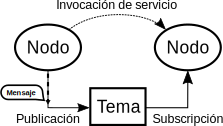
\includegraphics[width=0.5\linewidth]{img/ROS_concepts}
	\caption{Diagrama de comunicación de ROS}
	\label{fig:rosconcepts}
\end{figure}

\subsection{Nodo (Node)}
En ROS (Robot Operating System), un nodo es una unidad básica de ejecución. Se trata de un proceso individual que realiza una tarea específica dentro del sistema robótico. Los nodos pueden encargarse de diversas funciones, como leer datos de sensores, controlar motores, procesar imágenes o ejecutar algoritmos de navegación, entre otros.

Cada nodo en ROS:

Se ejecuta de forma independiente.

Se comunica con otros nodos mediante tópicos, servicios o acciones.

Puede estar programado en lenguajes compatibles con ROS, como Python o C++.

Es modular, lo que permite dividir un sistema complejo en componentes más manejables y reutilizables.

Por ejemplo, en un robot móvil, podría haber un nodo encargado de leer datos del LIDAR, otro que realice el mapeo del entorno, y otro que se encargue de la planificación de trayectorias. Todos estos nodos trabajan en conjunto mediante la infraestructura de comunicación de ROS.

En resumen, un nodo en ROS es un proceso que cumple una función específica dentro de un sistema robótico, facilitando la construcción de arquitecturas distribuidas, escalables y flexibles.

\subsection{Tema (Topic)}
En ROS, un topic representa un canal de comunicación que permite la transmisión de mensajes entre nodos de forma desacoplada y asincrónica. Es uno de los mecanismos fundamentales para el intercambio de información dentro del sistema. Los nodos pueden actuar como publicadores, enviando información a un topic determinado, o como suscriptores, recibiendo información publicada en ese mismo canal. Esto permite que múltiples nodos intercambien información sin necesidad de conocerse entre sí ni mantener una conexión directa.

Este mecanismo es particularmente útil para flujos de datos continuos y en tiempo real, como los que provienen de sensores (cámaras, LIDAR, IMU) o de módulos de control (por ejemplo, el movimiento de un robot móvil). Por ejemplo, un nodo que maneja un sensor LIDAR podría publicar datos en un topic llamado /scan, y un nodo de navegación podría suscribirse a ese topic para usar los datos y generar un mapa del entorno.

El sistema de topics favorece la escalabilidad, ya que múltiples nodos pueden suscribirse al mismo topic sin afectar al publicador. Además, ROS proporciona herramientas como rostopic list, rostopic echo y rqt_graph para monitorear y depurar estas comunicaciones en tiempo real.

\subsection{Mensaje (Message)}
Un mensaje en ROS es una estructura de datos que se transmite entre nodos a través de un topic. Cada mensaje tiene un tipo definido y puede contener campos de datos básicos como enteros, flotantes, booleanos, cadenas de texto, o estructuras más complejas como vectores, posiciones 3D, matrices, etc. Estos mensajes están definidos en archivos .msg, lo que permite mantener una estructura estándar y reutilizable.

Los mensajes garantizan la interoperabilidad entre nodos escritos en diferentes lenguajes de programación (como C++ o Python), ya que ROS maneja la serialización y deserialización automáticamente.

\subsection{Servicio (Service)}
A diferencia de los topics, que están diseñados para comunicaciones unidireccionales y continuas, los servicios en ROS están diseñados para interacciones bidireccionales y sincrónicas, donde se espera una respuesta específica tras una solicitud. Siguen el modelo cliente-servidor, donde un nodo cliente envía una solicitud (request) a un nodo servidor, el cual procesa la solicitud y devuelve una respuesta (response).

Los servicios se definen en archivos .srv, donde se especifican los campos del request y del response, separados por ---. Al igual que con los mensajes, ROS incluye varios servicios predefinidos, y también permite crear servicios personalizados.

Una limitación importante de los servicios es que son bloqueantes: el cliente debe esperar la respuesta antes de continuar con su ejecución, lo cual puede ser una desventaja en aplicaciones que requieren alta velocidad de respuesta o concurrencia.

\subsection{Gazebo}
Gazebo es un potente simulador robótico 3D de código abierto que permite simular entornos físicos complejos y robots en tiempo real con una alta fidelidad física. Gracias a su integración con ROS, es posible simular el comportamiento de robots reales sin necesidad de contar con el hardware físico, lo cual es ideal para desarrollo, prueba y validación de algoritmos de navegación, percepción, planificación de trayectorias y control.

Gazebo puede simular sensores como cámaras RGB y de profundidad, IMUs, LIDARs, GPS, y también puede emular diferentes tipos de terrenos, obstáculos y condiciones ambientales. Utiliza motores de física como ODE (Open Dynamics Engine) o Bullet para calcular interacciones físicas, colisiones, fricción, gravedad, etc.

\subsection{RViz}
RViz (ROS Visualization) es una herramienta gráfica interactiva de ROS que permite visualizar, en un espacio tridimensional, la información que fluye dentro del sistema robótico. Esto incluye visualizaciones del modelo del robot, datos de sensores (como cámaras, LIDAR, mapas), marcos de referencia (tf), trayectorias planificadas, objetivos de navegación, y mucho más.

RViz es fundamental durante el desarrollo de sistemas en ROS porque permite entender cómo el robot “percibe” su entorno y cómo está reaccionando ante diferentes situaciones. Los desarrolladores pueden depurar problemas, validar resultados y ajustar configuraciones directamente desde la interfaz.

La visualización se organiza en "Displays", que son módulos que se pueden añadir o quitar según las necesidades. Por ejemplo, un display de tipo LaserScan puede mostrar la información de un sensor LIDAR, mientras que uno de tipo Path puede mostrar la ruta que el robot planea seguir.

Además, RViz permite la interacción con el sistema, como seleccionar metas de navegación mediante clics o visualizar el resultado de algoritmos de detección de objetos, todo en tiempo real.

